\documentclass{article}
\usepackage{blindtext}
\usepackage{booktabs}
\usepackage[margin=0.25in]{geometry}
\usepackage{subcaption}
\usepackage{graphicx}
\usepackage{caption}
\usepackage{hyperref}
\usepackage{pdflscape}
\usepackage{tikz}


\title{Descriptive Tables and Figures for Municipality Proliferation}

\begin{document}
\maketitle
\tableofcontents
{\footnotesize 
\listoffigures
\listoftables}
\clearpage

\section{Land Use}
\begin{table}[htbp]\centering
\def\sym#1{\ifmmode^{#1}\else\(^{#1}\)\fi}
\caption{ \label{tab1}}
\begin{tabular}{l*{4}{c}}
\toprule
                    &\multicolumn{1}{c}{Full Sample}&\multicolumn{1}{c}{Northern Sample}&\multicolumn{1}{c}{Full Sample, pre-1940}&\multicolumn{1}{c}{Northern Sample, pre-1940}\\
\midrule
Local Political Pressure Index, 2018&      0.0110         &    -0.00324         &      0.0408         &      0.0348         \\
                    &      (0.07)         &     (-0.02)         &      (0.26)         &      (0.21)         \\
\addlinespace
State Political Involvement Index, 2018&       0.127         &       0.192\sym{*}  &       0.174         &       0.236\sym{*}  \\
                    &      (1.40)         &      (2.03)         &      (1.90)         &      (2.48)         \\
\addlinespace
Local Project Approval Index, 2018&      -0.147         &      -0.122         &      -0.132         &      -0.114         \\
                    &     (-1.36)         &     (-1.07)         &     (-1.21)         &     (-0.99)         \\
\addlinespace
Local Zoning Approval Index, 2018&      -0.214\sym{*}  &      -0.178         &      -0.225\sym{*}  &      -0.198         \\
                    &     (-2.03)         &     (-1.62)         &     (-2.12)         &     (-1.77)         \\
\addlinespace
Supply Restrictions Index, 2018&      0.0450         &      0.0207         &      0.0546         &      0.0108         \\
                    &      (0.67)         &      (0.29)         &      (0.81)         &      (0.15)         \\
\addlinespace
Density Restriction Index, 2018&      0.0131         &      0.0167         &      0.0962         &       0.100         \\
                    &      (0.14)         &      (0.17)         &      (1.01)         &      (1.00)         \\
\addlinespace
Exactions Index, 2018&      0.0644         &      0.0253         &      0.0819\sym{*}  &      0.0413         \\
                    &      (1.70)         &      (0.63)         &      (2.14)         &      (1.02)         \\
\addlinespace
Affordable Housing Index, 2018&      0.0340         &     0.00937         &      0.0329         &      0.0131         \\
                    &      (1.20)         &      (0.31)         &      (1.15)         &      (0.43)         \\
\addlinespace
Approval Delay Index, 2018&       1.326\sym{***}&       0.553         &       1.557\sym{***}&       0.847\sym{*}  \\
                    &      (4.25)         &      (1.63)         &      (5.01)         &      (2.50)         \\
\addlinespace
WRLURI 2018         &      0.0899         &      0.0321         &       0.138         &      0.0831         \\
                    &      (1.14)         &      (0.39)         &      (1.73)         &      (0.98)         \\
\midrule
Observations        &                     &                     &                     &                     \\
\bottomrule
\multicolumn{5}{l}{\footnotesize Unweighted}\\
\multicolumn{5}{l}{\footnotesize \sym{*} \(p<0.05\), \sym{**} \(p<0.01\), \sym{***} \(p<0.001\)}\\
\end{tabular}
\end{table}

\clearpage
\begin{table}[htbp]\centering
\def\sym#1{\ifmmode^{#1}\else\(^{#1}\)\fi}
\caption{ \label{tab1}}
\begin{tabular}{l*{4}{c}}
\toprule
                    &\multicolumn{1}{c}{Full Sample}&\multicolumn{1}{c}{Northern Sample}&\multicolumn{1}{c}{Full Sample, pre-1940}&\multicolumn{1}{c}{Northern Sample, pre-1940}\\
\midrule
Local Political Pressure Index, 2018&      -0.326         &      -0.326         &      -0.326         &      -0.326         \\
                    &     (-1.83)         &     (-1.90)         &     (-1.78)         &     (-1.85)         \\
\addlinespace
State Political Involvement Index, 2018&      0.0786         &      0.0786         &      0.0836         &      0.0836         \\
                    &      (0.82)         &      (0.85)         &      (0.86)         &      (0.89)         \\
\addlinespace
Local Project Approval Index, 2018&       0.109         &       0.109         &       0.116         &       0.116         \\
                    &      (0.89)         &      (0.92)         &      (0.91)         &      (0.95)         \\
\addlinespace
Local Zoning Approval Index, 2018&     -0.0511         &     -0.0511         &     -0.0879         &     -0.0879         \\
                    &     (-0.44)         &     (-0.45)         &     (-0.76)         &     (-0.79)         \\
\addlinespace
Supply Restrictions Index, 2018&      0.0202         &      0.0202         &     -0.0170         &     -0.0170         \\
                    &      (0.25)         &      (0.26)         &     (-0.20)         &     (-0.20)         \\
\addlinespace
Density Restriction Index, 2018&      -0.128         &      -0.128         &    -0.00747         &    -0.00747         \\
                    &     (-1.09)         &     (-1.13)         &     (-0.06)         &     (-0.07)         \\
\addlinespace
Exactions Index, 2018&     -0.0840\sym{*}  &     -0.0840\sym{*}  &     -0.0902\sym{*}  &     -0.0902\sym{*}  \\
                    &     (-2.16)         &     (-2.24)         &     (-2.24)         &     (-2.32)         \\
\addlinespace
Affordable Housing Index, 2018&    0.000173         &    0.000173         &     0.00194         &     0.00194         \\
                    &      (0.01)         &      (0.01)         &      (0.06)         &      (0.07)         \\
\addlinespace
Approval Delay Index, 2018&     -0.0377         &     -0.0377         &       0.287         &       0.287         \\
                    &     (-0.11)         &     (-0.11)         &      (0.82)         &      (0.85)         \\
\addlinespace
WRLURI 2018         &     -0.0870         &     -0.0870         &     -0.0680         &     -0.0680         \\
                    &     (-1.08)         &     (-1.12)         &     (-0.82)         &     (-0.85)         \\
\midrule
Observations        &                     &                     &                     &                     \\
\bottomrule
\multicolumn{5}{l}{\footnotesize Unweighted}\\
\multicolumn{5}{l}{\footnotesize \sym{*} \(p<0.05\), \sym{**} \(p<0.01\), \sym{***} \(p<0.001\)}\\
\end{tabular}
\end{table}

\clearpage
\begin{table}[htbp]\centering
\def\sym#1{\ifmmode^{#1}\else\(^{#1}\)\fi}
\caption{ \label{tab1}}
\begin{tabular}{l*{4}{c}}
\toprule
                    &\multicolumn{1}{c}{Full Sample}&\multicolumn{1}{c}{Northern Sample}&\multicolumn{1}{c}{Full Sample, pre-1940}&\multicolumn{1}{c}{Northern Sample, pre-1940}\\
\midrule
Local Political Pressure Index, 2018&      0.0265         &       0.100         &      0.0413         &       0.116         \\
                    &      (0.16)         &      (0.56)         &      (0.24)         &      (0.64)         \\
\addlinespace
State Political Involvement Index, 2018&      0.0767         &       0.168         &       0.120         &       0.201\sym{*}  \\
                    &      (0.85)         &      (1.78)         &      (1.32)         &      (2.11)         \\
\addlinespace
Local Project Approval Index, 2018&      -0.119         &      -0.125         &      -0.109         &     -0.0998         \\
                    &     (-1.00)         &     (-0.97)         &     (-0.91)         &     (-0.79)         \\
\addlinespace
Local Zoning Approval Index, 2018&      -0.264\sym{*}  &      -0.243\sym{*}  &      -0.282\sym{*}  &      -0.255\sym{*}  \\
                    &     (-2.36)         &     (-2.04)         &     (-2.49)         &     (-2.10)         \\
\addlinespace
Supply Restrictions Index, 2018&      0.0157         &    -0.00992         &      0.0294         &     -0.0205         \\
                    &      (0.24)         &     (-0.14)         &      (0.45)         &     (-0.28)         \\
\addlinespace
Density Restriction Index, 2018&      0.0118         &     -0.0103         &       0.101         &      0.0941         \\
                    &      (0.12)         &     (-0.10)         &      (1.00)         &      (0.90)         \\
\addlinespace
Exactions Index, 2018&      0.0845\sym{*}  &      0.0540         &      0.0960\sym{*}  &      0.0715         \\
                    &      (2.00)         &      (1.21)         &      (2.25)         &      (1.58)         \\
\addlinespace
Affordable Housing Index, 2018&      0.0339         &      0.0274         &      0.0357         &      0.0340         \\
                    &      (1.18)         &      (0.91)         &      (1.23)         &      (1.13)         \\
\addlinespace
Approval Delay Index, 2018&       1.455\sym{***}&       0.895\sym{**} &       1.641\sym{***}&       1.118\sym{***}\\
                    &      (4.80)         &      (2.76)         &      (5.39)         &      (3.44)         \\
\addlinespace
WRLURI 2018         &      0.0809         &      0.0549         &       0.127         &       0.108         \\
                    &      (1.00)         &      (0.64)         &      (1.55)         &      (1.25)         \\
\midrule
Observations        &                     &                     &                     &                     \\
\bottomrule
\multicolumn{5}{l}{\footnotesize Weight, full sample}\\
\multicolumn{5}{l}{\footnotesize \sym{*} \(p<0.05\), \sym{**} \(p<0.01\), \sym{***} \(p<0.001\)}\\
\end{tabular}
\end{table}

\clearpage
\begin{table}[htbp]\centering
\def\sym#1{\ifmmode^{#1}\else\(^{#1}\)\fi}
\caption{ \label{tab1}}
\begin{tabular}{l*{6}{c}}
\toprule
                    &\multicolumn{1}{c}{Full Sample}&\multicolumn{1}{c}{Northern Sample}&\multicolumn{1}{c}{Full Sample, pre-1970}&\multicolumn{1}{c}{Northern Sample, pre-1970}&\multicolumn{1}{c}{Dest Sample}&\multicolumn{1}{c}{Dest Sample, pre-1970}\\
\midrule
Local Political Pressure Index, 2018&      -0.267         &      -0.267         &      -0.303         &      -0.303         &      -0.267         &      -0.303         \\
                    &     (-1.76)         &     (-1.75)         &     (-1.91)         &     (-1.90)         &     (-1.75)         &     (-1.90)         \\
\addlinespace
State Political Involvement Index, 2018&      0.0583         &      0.0583         &      0.0503         &      0.0503         &      0.0583         &      0.0503         \\
                    &      (0.87)         &      (0.87)         &      (0.72)         &      (0.72)         &      (0.87)         &      (0.72)         \\
\addlinespace
Local Project Approval Index, 2018&       0.139         &       0.139         &       0.157         &       0.157         &       0.139         &       0.157         \\
                    &      (1.33)         &      (1.33)         &      (1.42)         &      (1.41)         &      (1.33)         &      (1.41)         \\
\addlinespace
Local Zoning Approval Index, 2018&      -0.116         &      -0.116         &      -0.143         &      -0.143         &      -0.116         &      -0.143         \\
                    &     (-1.20)         &     (-1.20)         &     (-1.53)         &     (-1.52)         &     (-1.20)         &     (-1.52)         \\
\addlinespace
Supply Restrictions Index, 2018&     -0.0127         &     -0.0127         &     -0.0583         &     -0.0583         &     -0.0127         &     -0.0583         \\
                    &     (-0.17)         &     (-0.17)         &     (-0.75)         &     (-0.75)         &     (-0.17)         &     (-0.75)         \\
\addlinespace
Density Restriction Index, 2018&      -0.199         &      -0.199         &     -0.0353         &     -0.0353         &      -0.199         &     -0.0353         \\
                    &     (-1.44)         &     (-1.44)         &     (-0.30)         &     (-0.30)         &     (-1.44)         &     (-0.30)         \\
\addlinespace
Exactions Index, 2018&     -0.0781         &     -0.0781         &     -0.0812         &     -0.0812         &     -0.0781         &     -0.0812         \\
                    &     (-1.60)         &     (-1.59)         &     (-1.52)         &     (-1.52)         &     (-1.59)         &     (-1.52)         \\
\addlinespace
Affordable Housing Index, 2018&     0.00531         &     0.00531         &      0.0119         &      0.0119         &     0.00531         &      0.0119         \\
                    &      (0.16)         &      (0.16)         &      (0.35)         &      (0.35)         &      (0.16)         &      (0.35)         \\
\addlinespace
Approval Delay Index, 2018&       0.127         &       0.127         &       0.327         &       0.327         &       0.127         &       0.327         \\
                    &      (0.31)         &      (0.31)         &      (0.98)         &      (0.98)         &      (0.31)         &      (0.98)         \\
\addlinespace
WRLURI 2018         &     -0.0934         &     -0.0934         &     -0.0733         &     -0.0733         &     -0.0934         &     -0.0733         \\
                    &     (-1.23)         &     (-1.23)         &     (-0.98)         &     (-0.98)         &     (-1.23)         &     (-0.98)         \\
\midrule
Observations        &                     &                     &                     &                     &                     &                     \\
\bottomrule
\multicolumn{7}{l}{\footnotesize Weight, full sample}\\
\multicolumn{7}{l}{\footnotesize \sym{*} \(p<0.05\), \sym{**} \(p<0.01\), \sym{***} \(p<0.001\)}\\
\end{tabular}
\end{table}

\clearpage
\begin{table}[htbp]\centering
\def\sym#1{\ifmmode^{#1}\else\(^{#1}\)\fi}
\caption{ \label{tab1}}
\begin{tabular}{l*{6}{c}}
\toprule
                    &\multicolumn{1}{c}{Full Sample}&\multicolumn{1}{c}{Northern Sample}&\multicolumn{1}{c}{Full Sample, pre-1970}&\multicolumn{1}{c}{Northern Sample, pre-1970}&\multicolumn{1}{c}{Dest Sample}&\multicolumn{1}{c}{Dest Sample, pre-1970}\\
\midrule
Local Political Pressure Index, 2018&    -0.00507         &      0.0848         &     0.00478         &       0.106         &      0.0848         &       0.106         \\
                    &     (-0.03)         &      (0.50)         &      (0.03)         &      (0.62)         &      (0.50)         &      (0.62)         \\
\addlinespace
State Political Involvement Index, 2018&      0.0723         &       0.184         &       0.115         &       0.224\sym{*}  &       0.184         &       0.224\sym{*}  \\
                    &      (0.78)         &      (1.89)         &      (1.22)         &      (2.28)         &      (1.89)         &      (2.28)         \\
\addlinespace
Local Project Approval Index, 2018&      -0.106         &      -0.117         &     -0.0835         &     -0.0843         &      -0.117         &     -0.0843         \\
                    &     (-0.89)         &     (-0.92)         &     (-0.70)         &     (-0.68)         &     (-0.92)         &     (-0.68)         \\
\addlinespace
Local Zoning Approval Index, 2018&      -0.209         &      -0.188         &      -0.231         &      -0.203         &      -0.188         &      -0.203         \\
                    &     (-1.76)         &     (-1.52)         &     (-1.92)         &     (-1.62)         &     (-1.52)         &     (-1.62)         \\
\addlinespace
Supply Restrictions Index, 2018&      0.0131         &    0.000347         &      0.0256         &     -0.0112         &    0.000347         &     -0.0112         \\
                    &      (0.19)         &      (0.00)         &      (0.36)         &     (-0.15)         &      (0.00)         &     (-0.15)         \\
\addlinespace
Density Restriction Index, 2018&     -0.0433         &     -0.0171         &      0.0507         &      0.0926         &     -0.0171         &      0.0926         \\
                    &     (-0.43)         &     (-0.16)         &      (0.50)         &      (0.88)         &     (-0.16)         &      (0.88)         \\
\addlinespace
Exactions Index, 2018&      0.0672         &      0.0397         &      0.0760         &      0.0561         &      0.0397         &      0.0561         \\
                    &      (1.64)         &      (0.92)         &      (1.83)         &      (1.28)         &      (0.92)         &      (1.28)         \\
\addlinespace
Affordable Housing Index, 2018&      0.0415         &      0.0234         &      0.0423         &      0.0301         &      0.0234         &      0.0301         \\
                    &      (1.39)         &      (0.75)         &      (1.40)         &      (0.96)         &      (0.75)         &      (0.96)         \\
\addlinespace
Approval Delay Index, 2018&       1.291\sym{***}&       0.776\sym{*}  &       1.479\sym{***}&       1.026\sym{**} &       0.776\sym{*}  &       1.026\sym{**} \\
                    &      (4.09)         &      (2.29)         &      (4.66)         &      (3.03)         &      (2.29)         &      (3.03)         \\
\addlinespace
WRLURI 2018         &      0.0618         &      0.0378         &       0.102         &      0.0947         &      0.0378         &      0.0947         \\
                    &      (0.75)         &      (0.43)         &      (1.22)         &      (1.07)         &      (0.43)         &      (1.07)         \\
\midrule
Observations        &                     &                     &                     &                     &                     &                     \\
\bottomrule
\multicolumn{7}{l}{\footnotesize Weight, metro sample}\\
\multicolumn{7}{l}{\footnotesize \sym{*} \(p<0.05\), \sym{**} \(p<0.01\), \sym{***} \(p<0.001\)}\\
\end{tabular}
\end{table}

\clearpage
\begin{table}[htbp]\centering
\def\sym#1{\ifmmode^{#1}\else\(^{#1}\)\fi}
\caption{ \label{tab1}}
\begin{tabular}{l*{4}{c}}
\toprule
                    &\multicolumn{1}{c}{Full Sample}&\multicolumn{1}{c}{Northern Sample}&\multicolumn{1}{c}{Full Sample, pre-1940}&\multicolumn{1}{c}{Northern Sample, pre-1940}\\
\midrule
Local Political Pressure Index, 2018&      -0.287         &      -0.287         &      -0.325         &      -0.325         \\
                    &     (-1.60)         &     (-1.64)         &     (-1.77)         &     (-1.82)         \\
\addlinespace
State Political Involvement Index, 2018&      0.0583         &      0.0583         &      0.0532         &      0.0532         \\
                    &      (0.58)         &      (0.59)         &      (0.52)         &      (0.54)         \\
\addlinespace
Local Project Approval Index, 2018&       0.180         &       0.180         &       0.191         &       0.191         \\
                    &      (1.35)         &      (1.38)         &      (1.38)         &      (1.42)         \\
\addlinespace
Local Zoning Approval Index, 2018&     -0.0597         &     -0.0597         &     -0.0901         &     -0.0901         \\
                    &     (-0.48)         &     (-0.49)         &     (-0.73)         &     (-0.75)         \\
\addlinespace
Supply Restrictions Index, 2018&    -0.00659         &    -0.00659         &     -0.0525         &     -0.0525         \\
                    &     (-0.08)         &     (-0.08)         &     (-0.61)         &     (-0.63)         \\
\addlinespace
Density Restriction Index, 2018&      -0.194         &      -0.194         &     -0.0321         &     -0.0321         \\
                    &     (-1.54)         &     (-1.58)         &     (-0.26)         &     (-0.26)         \\
\addlinespace
Exactions Index, 2018&     -0.0733         &     -0.0733         &     -0.0766         &     -0.0766         \\
                    &     (-1.76)         &     (-1.81)         &     (-1.76)         &     (-1.81)         \\
\addlinespace
Affordable Housing Index, 2018&     0.00636         &     0.00636         &      0.0125         &      0.0125         \\
                    &      (0.20)         &      (0.20)         &      (0.39)         &      (0.41)         \\
\addlinespace
Approval Delay Index, 2018&     -0.0294         &     -0.0294         &       0.240         &       0.240         \\
                    &     (-0.08)         &     (-0.08)         &      (0.67)         &      (0.69)         \\
\addlinespace
WRLURI 2018         &     -0.0931         &     -0.0931         &     -0.0726         &     -0.0726         \\
                    &     (-1.10)         &     (-1.12)         &     (-0.82)         &     (-0.85)         \\
\midrule
Observations        &                     &                     &                     &                     \\
\bottomrule
\multicolumn{5}{l}{\footnotesize Weight, metro sample}\\
\multicolumn{5}{l}{\footnotesize \sym{*} \(p<0.05\), \sym{**} \(p<0.01\), \sym{***} \(p<0.001\)}\\
\end{tabular}
\end{table}

\clearpage

\begin{table}[htbp]\centering
\def\sym#1{\ifmmode^{#1}\else\(^{#1}\)\fi}
\caption{ \label{tab1}}
\begin{tabular}{l*{4}{c}}
\toprule
                    &\multicolumn{1}{c}{Full Sample}&\multicolumn{1}{c}{Northern Sample}&\multicolumn{1}{c}{Full Sample, pre-1940}&\multicolumn{1}{c}{Northern Sample, pre-1940}\\
\midrule
landuse\_sfr         &      0.0499\sym{***}&      0.0271\sym{***}&      0.0389\sym{***}&      0.0237\sym{**} \\
                    &      (6.31)         &      (3.35)         &      (4.84)         &      (2.87)         \\
\addlinespace
landuse\_townhouse   &     0.00531\sym{**} &   -0.000838         &     0.00675\sym{***}&     0.00283         \\
                    &      (2.95)         &     (-0.44)         &      (3.73)         &      (1.49)         \\
\addlinespace
landuse\_residentialnec&     -0.0444\sym{***}&     -0.0197\sym{**} &     -0.0573\sym{***}&     -0.0299\sym{***}\\
                    &     (-6.22)         &     (-2.70)         &     (-7.86)         &     (-3.98)         \\
\addlinespace
landuse\_duplex      &    -0.00243\sym{**} &     -0.0121\sym{***}&    -0.00491\sym{***}&     -0.0149\sym{***}\\
                    &     (-2.65)         &    (-11.86)         &     (-5.18)         &    (-13.41)         \\
\addlinespace
landuse\_apartment   &     0.00154\sym{*}  &    -0.00105         &    0.000330         &    -0.00243\sym{***}\\
                    &      (2.38)         &     (-1.55)         &      (0.51)         &     (-3.61)         \\
\addlinespace
landuse\_condo       &      0.0356\sym{***}&      0.0255\sym{***}&      0.0385\sym{***}&      0.0281\sym{***}\\
                    &      (9.61)         &      (6.76)         &     (10.36)         &      (7.40)         \\
\addlinespace
landuse\_multifam    &    -0.00126\sym{**} &    -0.00173\sym{***}&    -0.00197\sym{***}&    -0.00209\sym{***}\\
                    &     (-2.93)         &     (-3.73)         &     (-4.49)         &     (-4.30)         \\
\addlinespace
landuse\_mobilehome  &     -0.0328\sym{***}&     -0.0103\sym{***}&     -0.0177\sym{***}&    -0.00465\sym{***}\\
                    &    (-24.39)         &     (-7.64)         &    (-13.41)         &     (-3.54)         \\
\addlinespace
landuse\_triplex     &    0.000102         &    -0.00150\sym{***}&   -0.000378         &    -0.00219\sym{***}\\
                    &      (0.35)         &     (-5.01)         &     (-1.29)         &     (-6.84)         \\
\midrule
Observations        &                     &                     &                     &                     \\
\bottomrule
\multicolumn{5}{l}{\footnotesize \textit{t} statistics in parentheses}\\
\multicolumn{5}{l}{\footnotesize Unweighted}\\
\multicolumn{5}{l}{\footnotesize Each value is a regression of the share of area zoned for a specific use on a dummy}\\
\multicolumn{5}{l}{\footnotesize for being a municipality incorporated between 1940-70 in one of the 130 destination CZs}\\
\multicolumn{5}{l}{\footnotesize \sym{*} \(p<0.05\), \sym{**} \(p<0.01\), \sym{***} \(p<0.001\)}\\
\end{tabular}
\end{table}

\clearpage
\begin{table}[htbp]\centering
\def\sym#1{\ifmmode^{#1}\else\(^{#1}\)\fi}
\caption{ \label{tab1}}
\begin{tabular}{l*{6}{c}}
\toprule
                    &\multicolumn{1}{c}{Full Sample}&\multicolumn{1}{c}{Northern Sample}&\multicolumn{1}{c}{Full Sample, pre-1970}&\multicolumn{1}{c}{Northern Sample, pre-1970}&\multicolumn{1}{c}{Dest Sample}&\multicolumn{1}{c}{Dest Sample, pre-1970}\\
\midrule
landuse\_sfr         &      0.0225         &      0.0234         &      0.0231         &      0.0241         &      0.0234         &      0.0241         \\
                    &      (1.56)         &      (1.59)         &      (1.72)         &      (1.75)         &      (1.59)         &      (1.75)         \\
\addlinespace
landuse\_townhouse   &     0.00489         &     0.00483         &     0.00477         &     0.00470         &     0.00483         &     0.00470         \\
                    &      (1.61)         &      (1.58)         &      (1.52)         &      (1.49)         &      (1.58)         &      (1.49)         \\
\addlinespace
landuse\_residentialnec&     -0.0237\sym{*}  &     -0.0248\sym{*}  &     -0.0242\sym{*}  &     -0.0254\sym{*}  &     -0.0248\sym{*}  &     -0.0254\sym{*}  \\
                    &     (-2.04)         &     (-2.07)         &     (-2.09)         &     (-2.11)         &     (-2.07)         &     (-2.11)         \\
\addlinespace
landuse\_duplex      &    -0.00479\sym{**} &    -0.00474\sym{**} &    -0.00604\sym{***}&    -0.00599\sym{***}&    -0.00474\sym{**} &    -0.00599\sym{***}\\
                    &     (-3.03)         &     (-2.99)         &     (-3.98)         &     (-3.93)         &     (-2.99)         &     (-3.93)         \\
\addlinespace
landuse\_apartment   &    -0.00117         &    -0.00119         &    -0.00142         &    -0.00142         &    -0.00119         &    -0.00142         \\
                    &     (-0.98)         &     (-0.98)         &     (-1.22)         &     (-1.21)         &     (-0.98)         &     (-1.21)         \\
\addlinespace
landuse\_condo       &     0.00918         &     0.00916         &      0.0108\sym{*}  &      0.0108\sym{*}  &     0.00916         &      0.0108\sym{*}  \\
                    &      (1.53)         &      (1.53)         &      (2.08)         &      (2.09)         &      (1.53)         &      (2.09)         \\
\addlinespace
landuse\_multifam    &    -0.00168\sym{**} &    -0.00172\sym{**} &    -0.00209\sym{**} &    -0.00216\sym{***}&    -0.00172\sym{**} &    -0.00216\sym{***}\\
                    &     (-2.86)         &     (-2.93)         &     (-3.27)         &     (-3.37)         &     (-2.93)         &     (-3.37)         \\
\addlinespace
landuse\_mobilehome  &    -0.00365\sym{*}  &    -0.00342\sym{*}  &    -0.00319         &    -0.00288         &    -0.00342\sym{*}  &    -0.00288         \\
                    &     (-2.11)         &     (-2.00)         &     (-1.95)         &     (-1.80)         &     (-2.00)         &     (-1.80)         \\
\addlinespace
landuse\_triplex     &   -0.000711\sym{**} &   -0.000702\sym{*}  &    -0.00105\sym{***}&    -0.00103\sym{**} &   -0.000702\sym{*}  &    -0.00103\sym{**} \\
                    &     (-2.60)         &     (-2.57)         &     (-3.31)         &     (-3.27)         &     (-2.57)         &     (-3.27)         \\
\midrule
Observations        &                     &                     &                     &                     &                     &                     \\
\bottomrule
\multicolumn{7}{l}{\footnotesize \textit{t} statistics in parentheses}\\
\multicolumn{7}{l}{\footnotesize Unweighted}\\
\multicolumn{7}{l}{\footnotesize Each value is a regression of the share of area zoned for a specific use on a dummy}\\
\multicolumn{7}{l}{\footnotesize for being a municipality incorporated between 1940-70 in one of the 130 destination CZs}\\
\multicolumn{7}{l}{\footnotesize Includes census region and CZ fixed effects}\\
\multicolumn{7}{l}{\footnotesize \sym{*} \(p<0.05\), \sym{**} \(p<0.01\), \sym{***} \(p<0.001\)}\\
\end{tabular}
\end{table}

\clearpage
\begin{table}[htbp]\centering
\def\sym#1{\ifmmode^{#1}\else\(^{#1}\)\fi}
\caption{ \label{tab1}}
\begin{tabular}{l*{4}{c}}
\toprule
                    &\multicolumn{1}{c}{Full Sample}&\multicolumn{1}{c}{Northern Sample}&\multicolumn{1}{c}{Full Sample, pre-1940}&\multicolumn{1}{c}{Northern Sample, pre-1940}\\
\midrule
landuse\_sfr         &      0.0477\sym{***}&      0.0473\sym{***}&      0.0229\sym{*}  &      0.0453\sym{***}\\
                    &      (4.31)         &      (3.92)         &      (1.99)         &      (3.33)         \\
\addlinespace
landuse\_townhouse   &     0.00794\sym{*}  &     0.00292         &     0.00574         &     0.00377         \\
                    &      (2.22)         &      (0.72)         &      (1.50)         &      (0.78)         \\
\addlinespace
landuse\_residentialnec&     -0.0394\sym{***}&     -0.0236\sym{***}&     -0.0339\sym{***}&     -0.0245\sym{***}\\
                    &     (-7.04)         &     (-3.83)         &     (-5.59)         &     (-3.39)         \\
\addlinespace
landuse\_duplex      &    -0.00459\sym{**} &     -0.0138\sym{***}&    -0.00991\sym{***}&     -0.0214\sym{***}\\
                    &     (-2.99)         &     (-6.78)         &     (-5.49)         &     (-7.63)         \\
\addlinespace
landuse\_apartment   &    -0.00112\sym{**} &    -0.00410\sym{***}&    -0.00318\sym{***}&    -0.00700\sym{***}\\
                    &     (-3.20)         &     (-7.02)         &     (-6.71)         &     (-8.03)         \\
\addlinespace
landuse\_condo       &      0.0343\sym{***}&      0.0168\sym{*}  &      0.0282\sym{***}&     0.00791         \\
                    &      (4.32)         &      (2.01)         &      (3.46)         &      (0.87)         \\
\addlinespace
landuse\_multifam    &    -0.00166\sym{***}&    -0.00202\sym{***}&    -0.00299\sym{***}&    -0.00301\sym{***}\\
                    &     (-3.60)         &     (-3.72)         &     (-5.78)         &     (-4.46)         \\
\addlinespace
landuse\_mobilehome  &     -0.0303\sym{***}&     -0.0119\sym{***}&    -0.00759\sym{**} &     0.00152         \\
                    &    (-11.97)         &     (-4.69)         &     (-3.21)         &      (0.76)         \\
\addlinespace
landuse\_triplex     &   -0.000570         &    -0.00301\sym{***}&    -0.00159\sym{***}&    -0.00494\sym{***}\\
                    &     (-1.84)         &     (-5.77)         &     (-3.83)         &     (-6.20)         \\
\midrule
Observations        &                     &                     &                     &                     \\
\bottomrule
\multicolumn{5}{l}{\footnotesize \textit{t} statistics in parentheses}\\
\multicolumn{5}{l}{\footnotesize Weighted by land area}\\
\multicolumn{5}{l}{\footnotesize Each value is a regression of the share of area zoned for a specific use on a dummy}\\
\multicolumn{5}{l}{\footnotesize for being a municipality incorporated between 1940-70 in one of the 130 destination CZs}\\
\multicolumn{5}{l}{\footnotesize \sym{*} \(p<0.05\), \sym{**} \(p<0.01\), \sym{***} \(p<0.001\)}\\
\end{tabular}
\end{table}

\clearpage
\begin{table}[htbp]\centering
\def\sym#1{\ifmmode^{#1}\else\(^{#1}\)\fi}
\caption{ \label{tab1}}
\begin{tabular}{l*{4}{c}}
\toprule
                    &\multicolumn{1}{c}{Full Sample}&\multicolumn{1}{c}{Northern Sample}&\multicolumn{1}{c}{Full Sample, pre-1940}&\multicolumn{1}{c}{Northern Sample, pre-1940}\\
\midrule
landuse\_sfr         &      0.0436\sym{***}&      0.0436\sym{***}&      0.0355\sym{**} &      0.0356\sym{**} \\
                    &      (3.48)         &      (3.51)         &      (2.85)         &      (2.90)         \\
\addlinespace
landuse\_townhouse   &     0.00621\sym{*}  &     0.00621\sym{*}  &     0.00290         &     0.00290         \\
                    &      (2.26)         &      (2.28)         &      (1.00)         &      (1.01)         \\
\addlinespace
landuse\_residentialnec&     -0.0148\sym{**} &     -0.0148\sym{**} &    -0.00796         &    -0.00810         \\
                    &     (-2.60)         &     (-2.64)         &     (-1.33)         &     (-1.37)         \\
\addlinespace
landuse\_duplex      &    -0.00666\sym{***}&    -0.00665\sym{***}&     -0.0124\sym{***}&     -0.0124\sym{***}\\
                    &     (-3.35)         &     (-3.38)         &     (-4.77)         &     (-4.83)         \\
\addlinespace
landuse\_apartment   &    -0.00261\sym{***}&    -0.00260\sym{***}&    -0.00560\sym{***}&    -0.00559\sym{***}\\
                    &     (-3.76)         &     (-3.78)         &     (-5.39)         &     (-5.46)         \\
\addlinespace
landuse\_condo       &     0.00638         &     0.00639         &    -0.00934         &    -0.00932         \\
                    &      (0.80)         &      (0.81)         &     (-1.07)         &     (-1.08)         \\
\addlinespace
landuse\_multifam    &    -0.00179\sym{*}  &    -0.00179\sym{*}  &    -0.00327\sym{***}&    -0.00328\sym{***}\\
                    &     (-2.54)         &     (-2.56)         &     (-3.81)         &     (-3.86)         \\
\addlinespace
landuse\_mobilehome  &     -0.0170\sym{***}&     -0.0170\sym{***}&    0.000810         &    0.000817         \\
                    &     (-4.15)         &     (-4.18)         &      (0.47)         &      (0.48)         \\
\addlinespace
landuse\_triplex     &    -0.00125\sym{**} &    -0.00125\sym{**} &    -0.00264\sym{***}&    -0.00264\sym{***}\\
                    &     (-2.80)         &     (-2.82)         &     (-4.34)         &     (-4.40)         \\
\midrule
Observations        &                     &                     &                     &                     \\
\bottomrule
\multicolumn{5}{l}{\footnotesize \textit{t} statistics in parentheses}\\
\multicolumn{5}{l}{\footnotesize Weighted by land area}\\
\multicolumn{5}{l}{\footnotesize Each value is a regression of the share of area zoned for a specific use on a dummy}\\
\multicolumn{5}{l}{\footnotesize for being a municipality incorporated between 1940-70 in one of the 130 destination CZs}\\
\multicolumn{5}{l}{\footnotesize Includes census region and CZ fixed effects}\\
\multicolumn{5}{l}{\footnotesize \sym{*} \(p<0.05\), \sym{**} \(p<0.01\), \sym{***} \(p<0.001\)}\\
\end{tabular}
\end{table}

\clearpage


\section{Distributions}
\begin{figure}
	\centering
	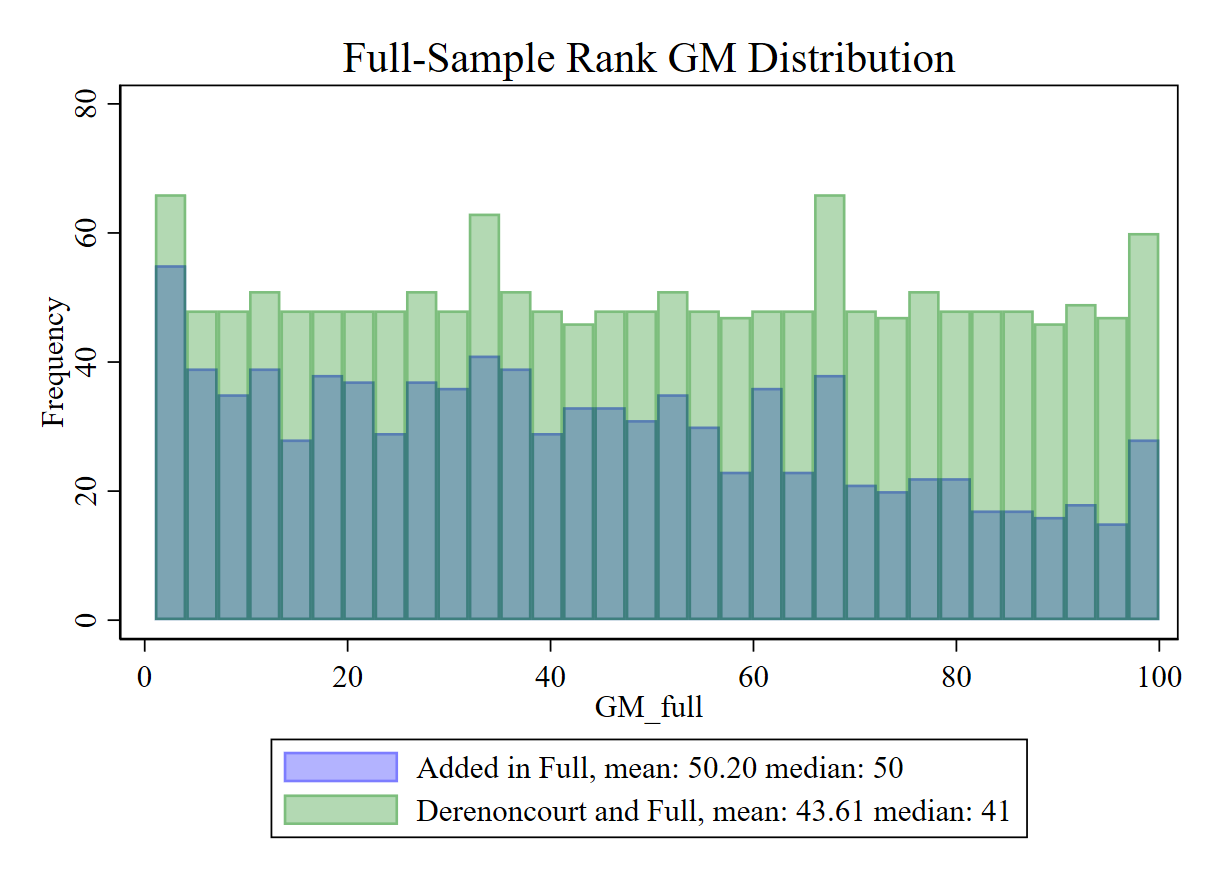
\includegraphics[width=.8\textwidth]{figures/distributions/GM_full.png}
\end{figure}
\clearpage
\begin{figure}
	\centering
	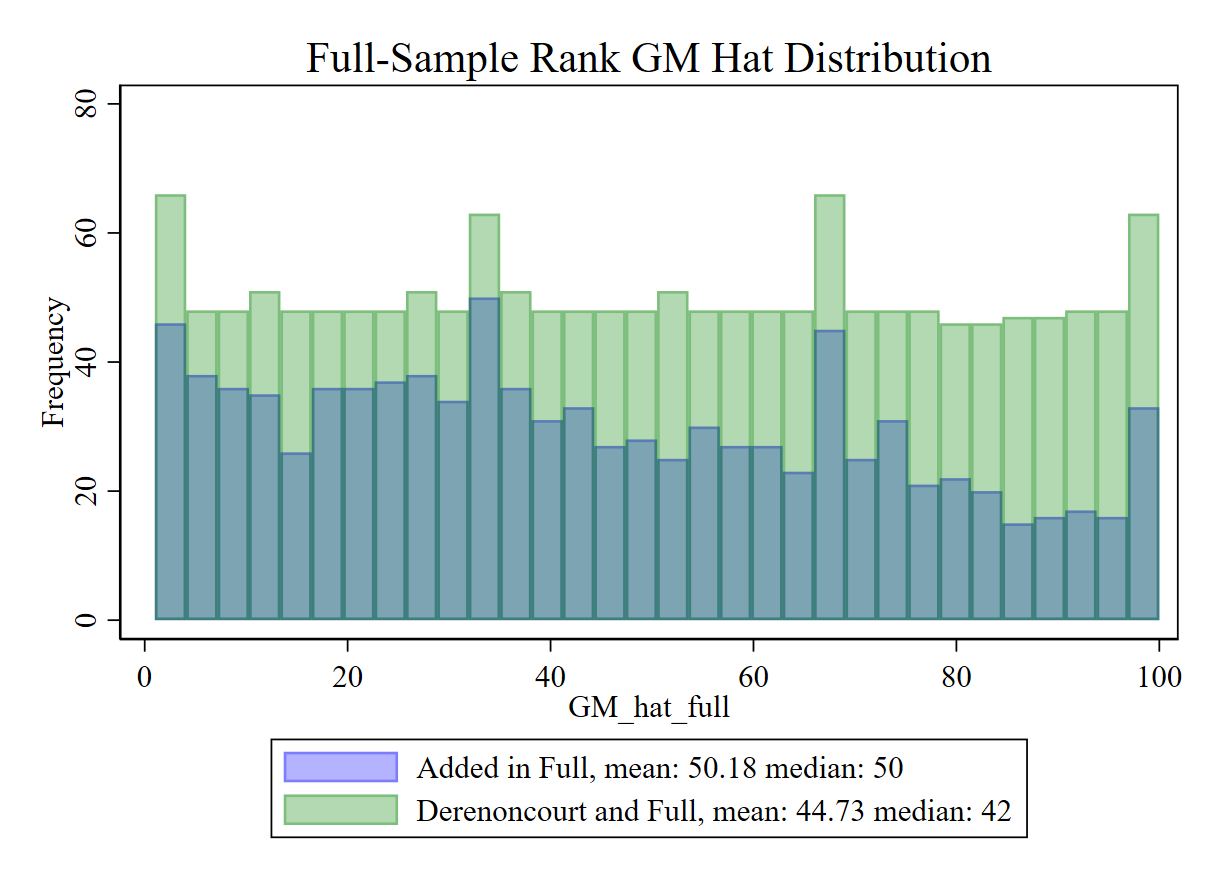
\includegraphics[width=.8\textwidth]{figures/distributions/GM_hat_full.png}
\end{figure}
\clearpage
\begin{figure}
	\centering
	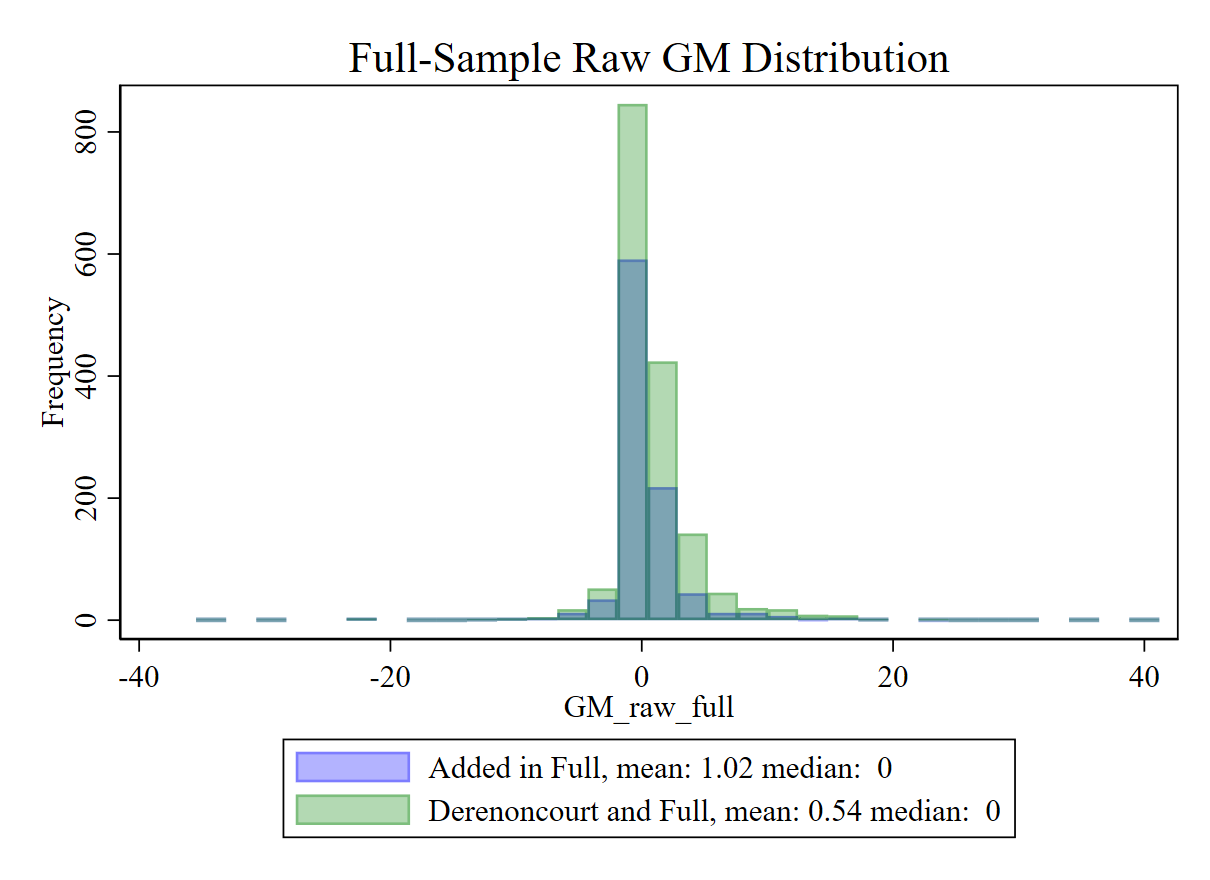
\includegraphics[width=.8\textwidth]{figures/distributions/GM_raw_full.png}
\end{figure}
\clearpage
\begin{figure}
	\centering
	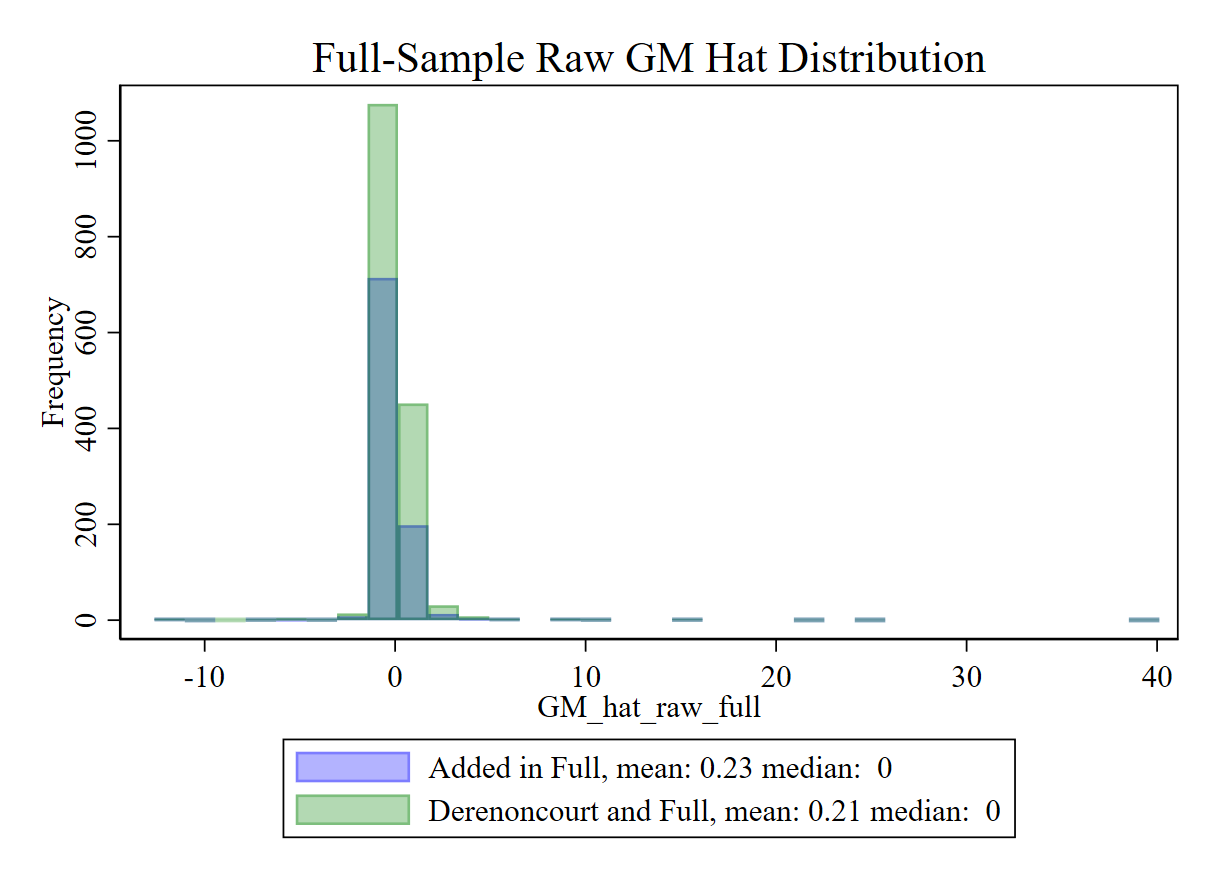
\includegraphics[width=.8\textwidth]{figures/distributions/GM_hat_raw_full.png}
\end{figure}
\clearpage
\begin{figure}
	\centering
	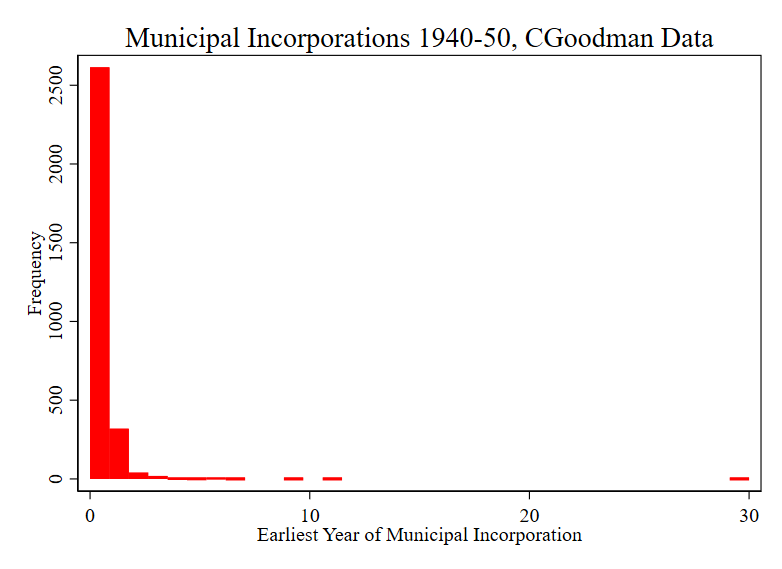
\includegraphics[width=.8\textwidth]{figures/distributions/cgoodman_1940.png}
	\caption{1940-50}
\end{figure}
\clearpage
\begin{figure}
	\centering
	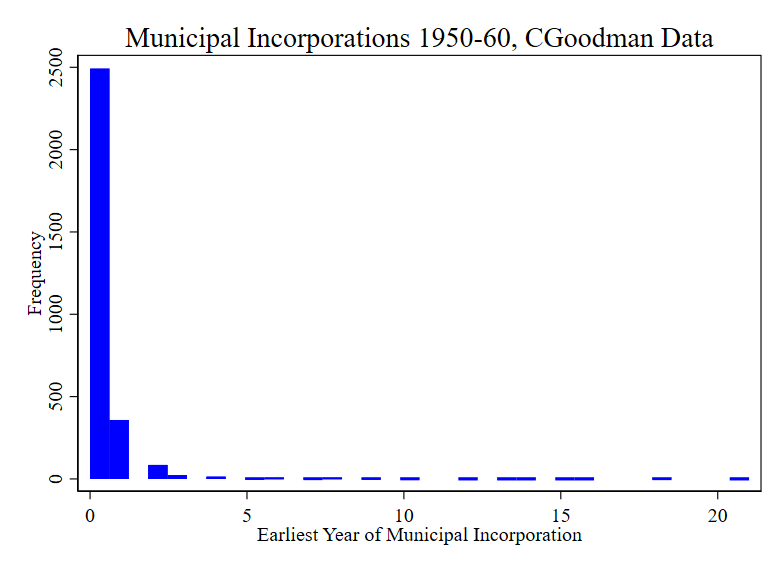
\includegraphics[width=.8\textwidth]{figures/distributions/cgoodman_1950.png}
	\caption{1950-60}
\end{figure}
\clearpage
\begin{figure}
	\centering
	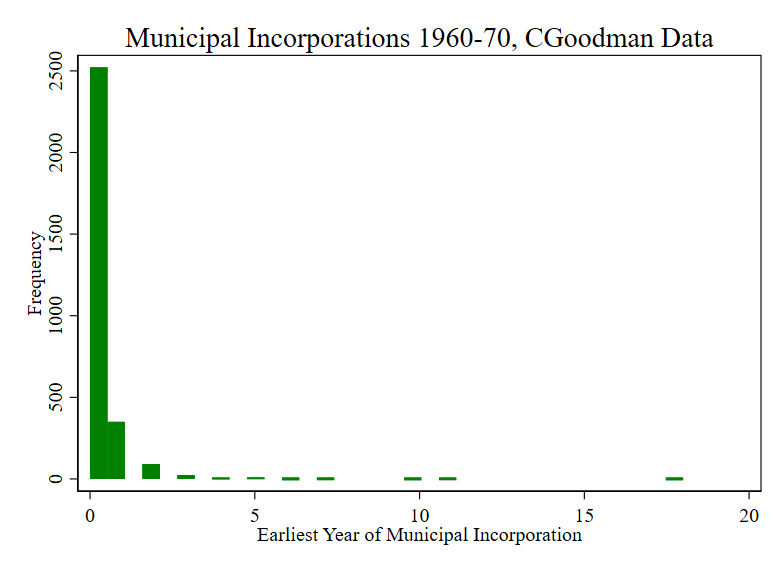
\includegraphics[width=.8\textwidth]{figures/distributions/cgoodman_1960.png}
	\caption{1960-70}
\end{figure}
\clearpage

\section{Jasper vs. Lake Counties}
\clearpage
\begin{figure}
	\centering
	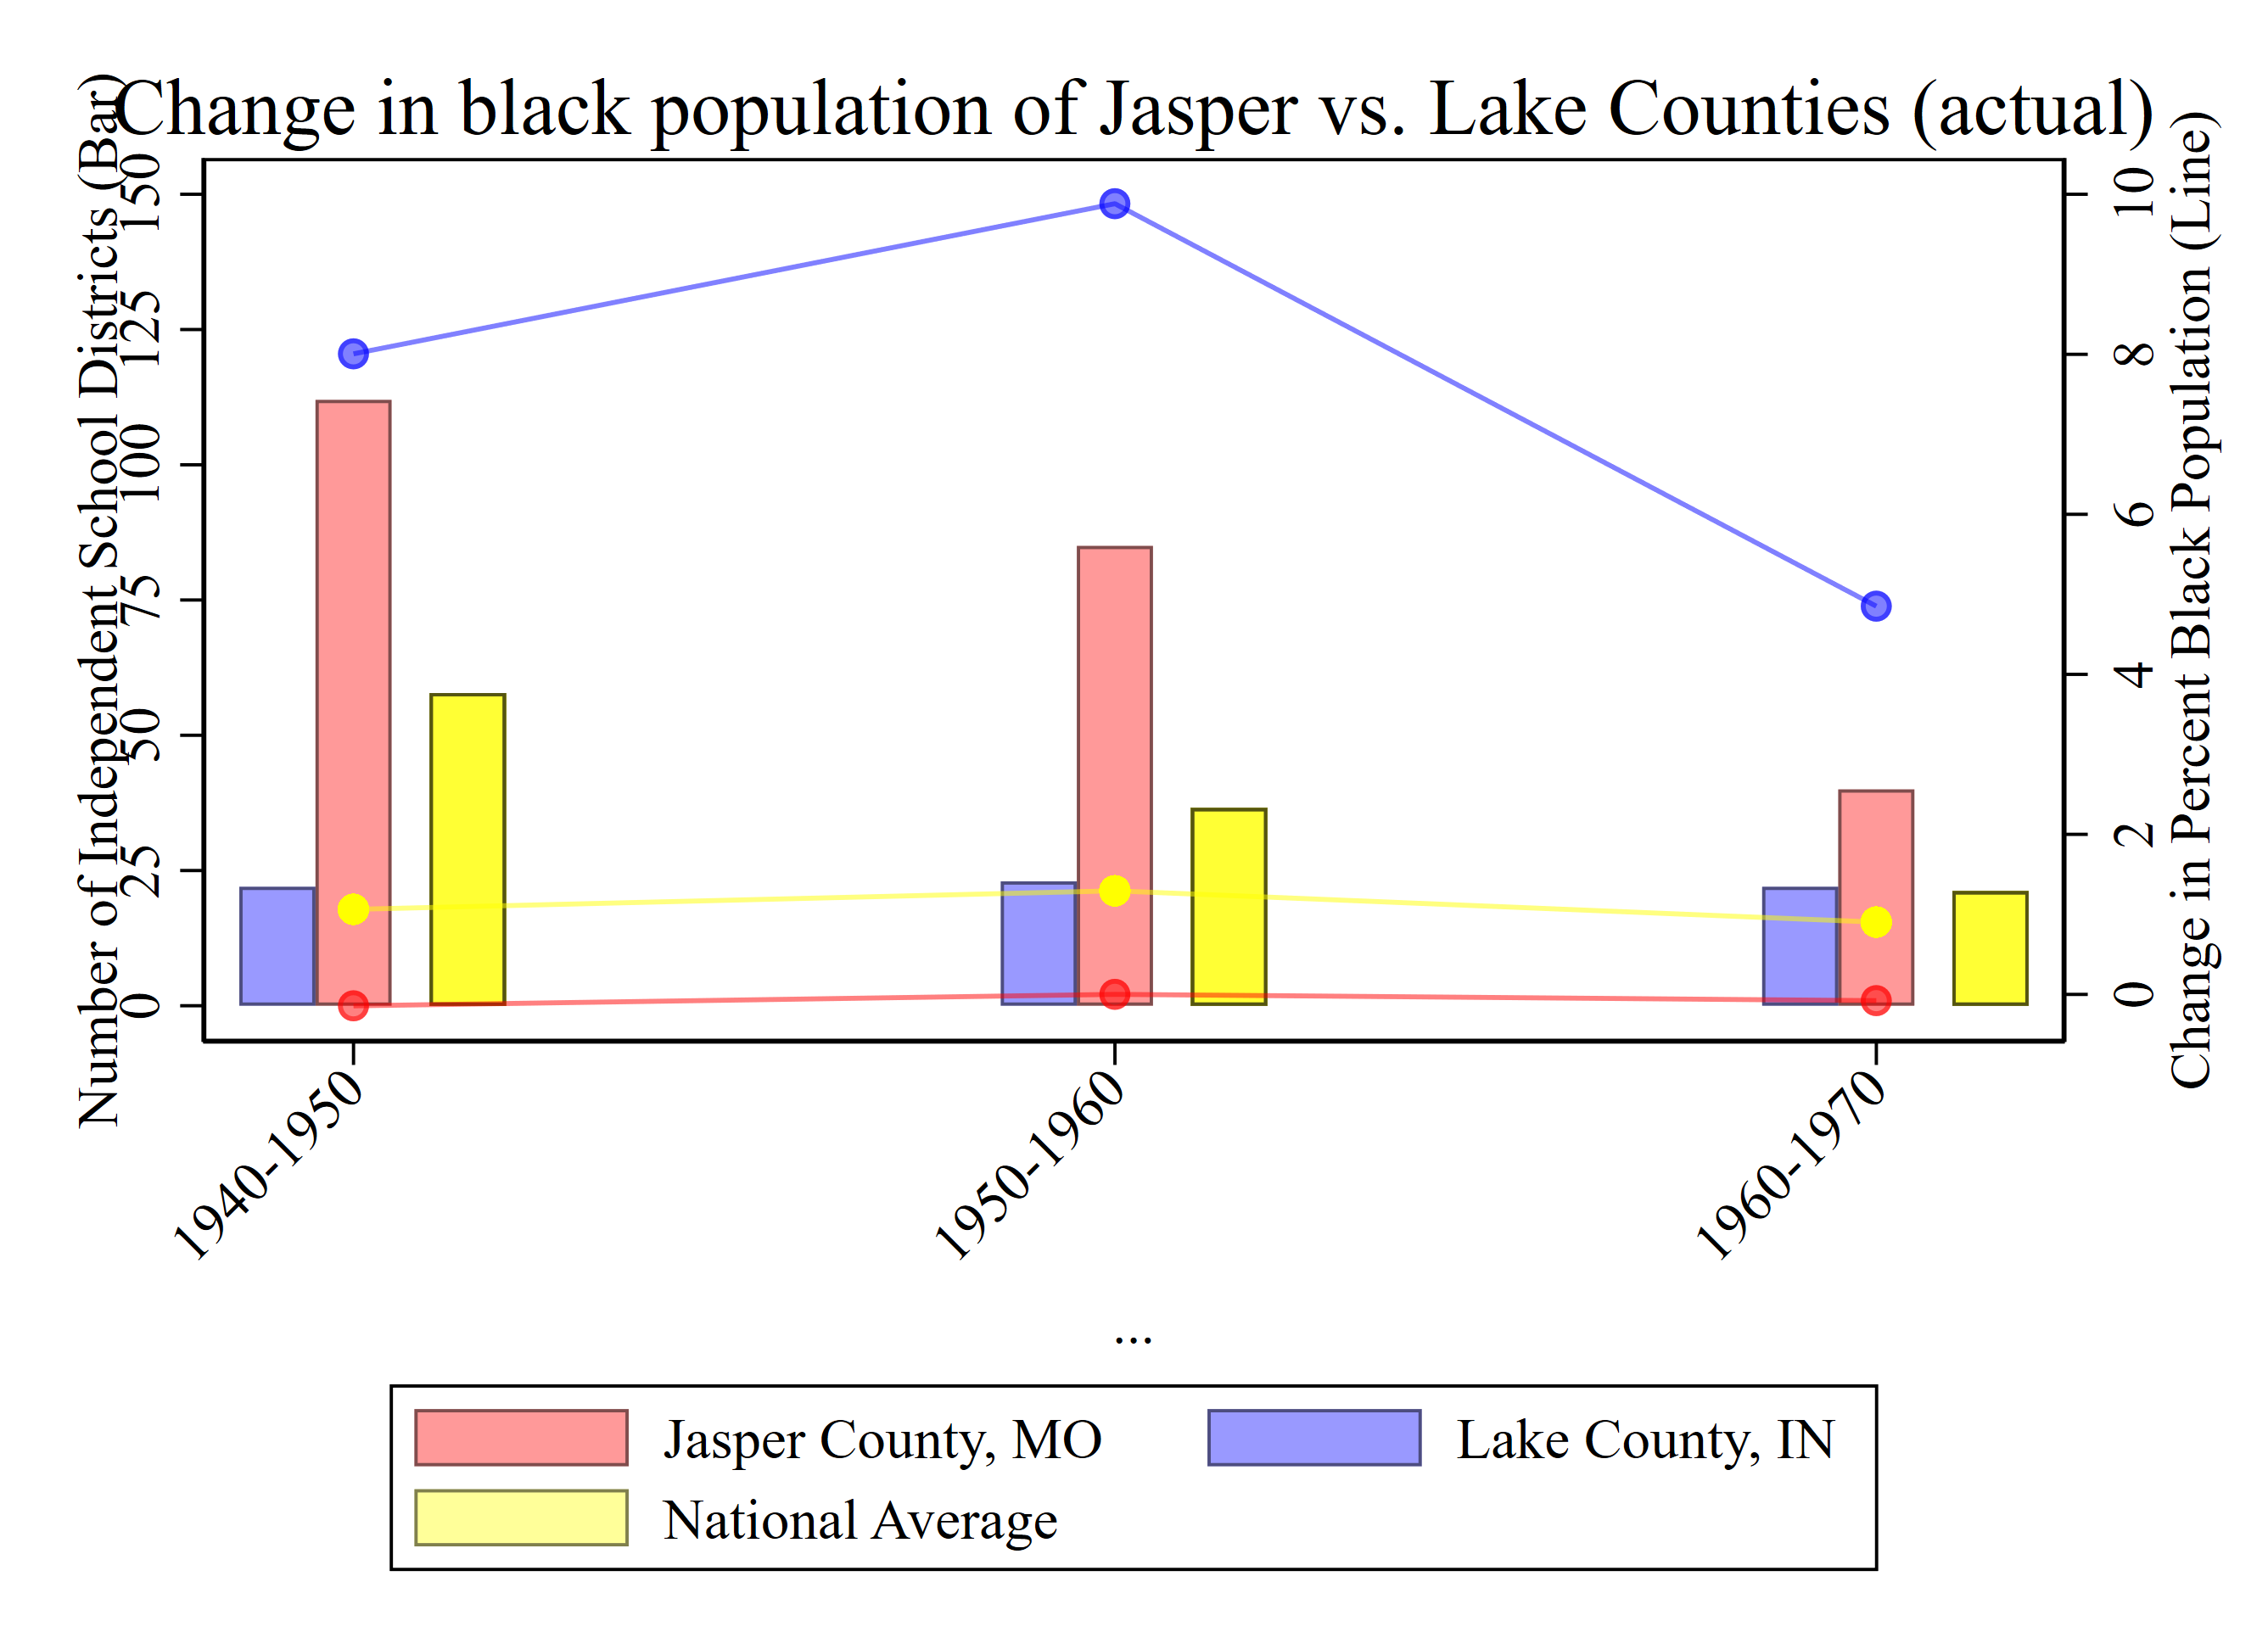
\includegraphics[width=.8\textwidth]{figures/descriptive/comparison.png}
\end{figure}
\clearpage
\begin{figure}
	\centering
	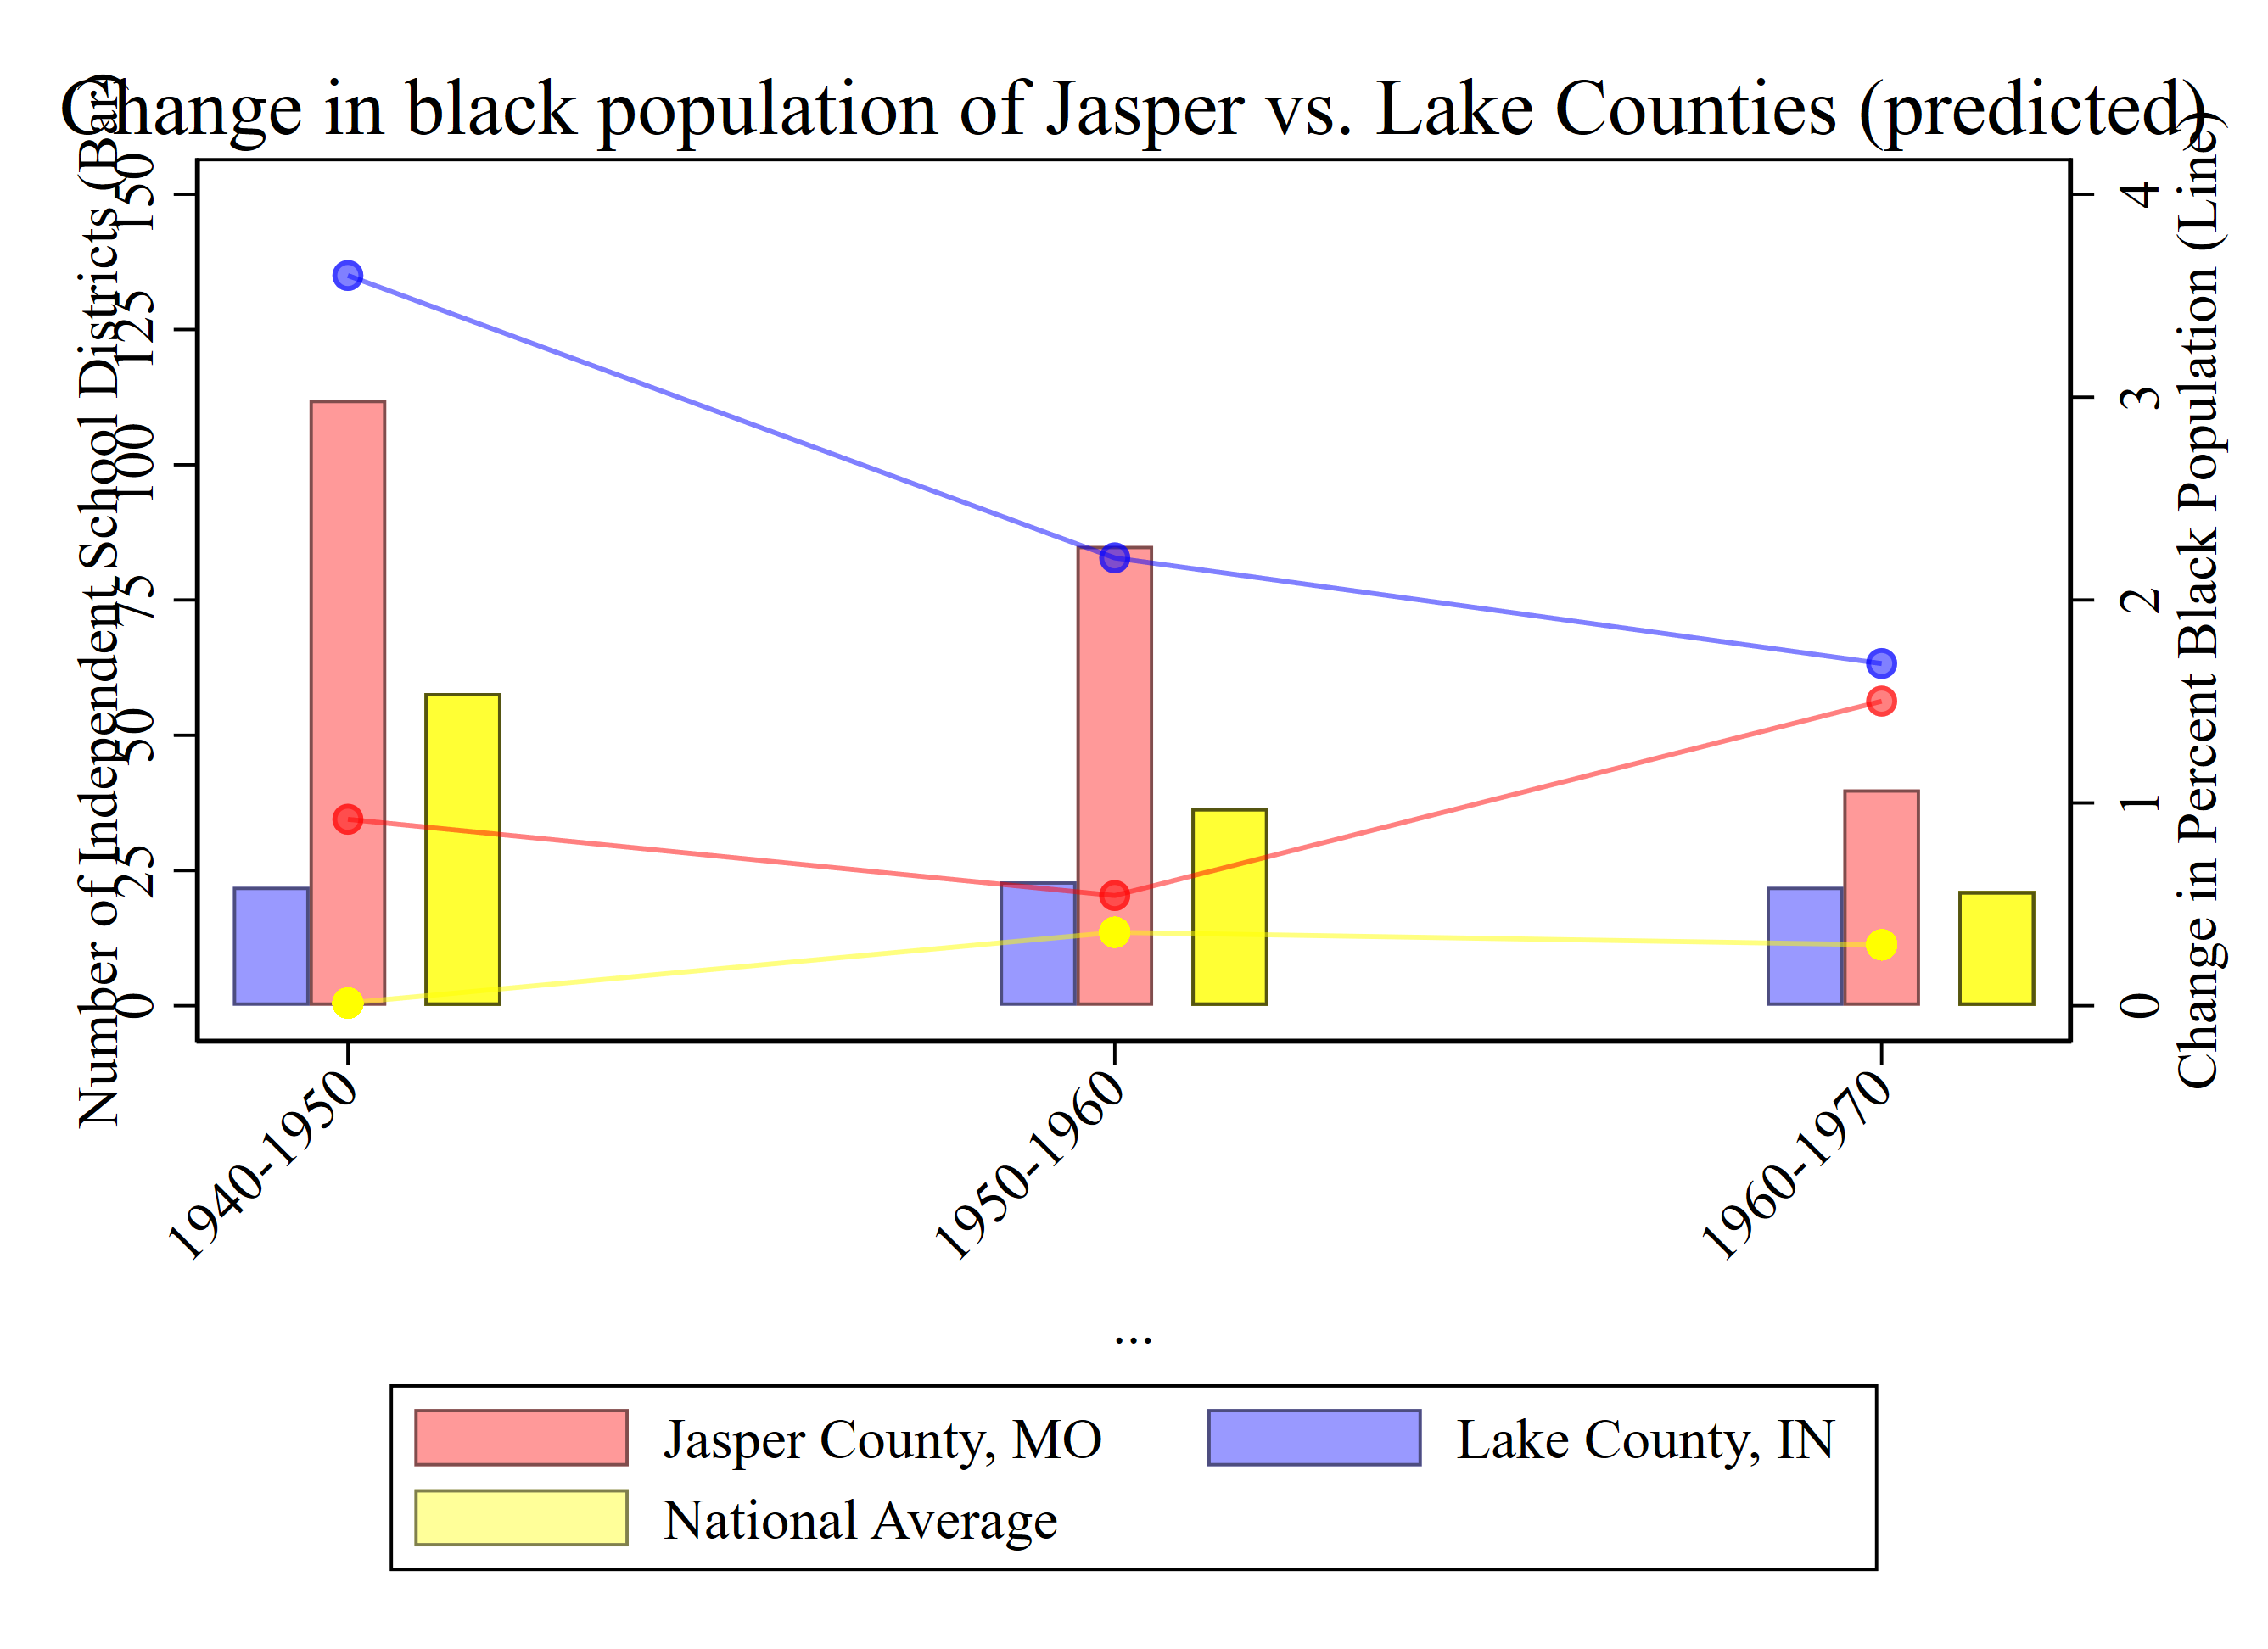
\includegraphics[width=.8\textwidth]{figures/descriptive/comparison_hat.png}
\end{figure}
\clearpage
\section{Goldsmith-Pinkham Table}
\begin{landscape}
{
\def\sym#1{\ifmmode^{#1}\else\(^{#1}\)\fi}
\begin{tabular}{l*{5}{c}}
\toprule
                &\multicolumn{3}{c}{County Counts Outcomes}  &\multicolumn{1}{c}{CGoodman Data}&\multicolumn{1}{c}{Instrument}\\\cmidrule(lr){2-4}\cmidrule(lr){5-5}\cmidrule(lr){6-6}
                &\multicolumn{1}{c}{n\_schdist\_ind\_cz\_pc}&\multicolumn{1}{c}{n\_gen\_subcounty\_cz\_pc}&\multicolumn{1}{c}{n\_gen\_muni\_cz\_pc}&\multicolumn{1}{c}{n\_cgoodman\_cz\_pc}&\multicolumn{1}{c}{GM\_hat\_raw\_pp}\\
\midrule
base\_outcome    &      -0.97***&      -0.22***&      -0.13*  &      -0.14** &              \\
                &     (0.01)   &     (0.04)   &     (0.07)   &     (0.06)   &              \\
\addlinespace
mfg\_lfshare1940 &      -0.35   &       0.38   &       0.25   &       0.19   &       0.08** \\
                &     (0.50)   &     (0.35)   &     (0.21)   &     (0.19)   &     (0.03)   \\
\addlinespace
blackmig3539\_share&     -15.14*  &       3.37   &      -5.64   &      -3.17   &      19.85***\\
                &     (7.94)   &    (11.55)   &     (8.60)   &     (6.28)   &     (5.45)   \\
\addlinespace
pop1940         &      -0.00*  &       0.00   &       0.00*  &       0.00   &       0.00** \\
                &     (0.00)   &     (0.00)   &     (0.00)   &     (0.00)   &     (0.00)   \\
\addlinespace
frac\_land       &     -23.87   &    -107.41** &     -37.28*  &     -33.92*  &      -3.79   \\
                &    (42.93)   &    (47.80)   &    (20.28)   &    (18.05)   &     (6.51)   \\
\addlinespace
reg2            &     -24.50** &     -30.33***&      -7.21** &      -7.50** &       2.31***\\
                &    (11.92)   &     (9.50)   &     (3.60)   &     (3.00)   &     (0.84)   \\
\addlinespace
reg3            &     -26.34*  &      -4.61   &      25.95   &      15.72   &       8.00** \\
                &    (15.10)   &    (21.53)   &    (19.48)   &    (12.48)   &     (3.61)   \\
\addlinespace
reg4            &     -20.49   &     -38.78***&     -10.23   &     -13.09** &      -1.69*  \\
                &    (18.93)   &    (11.90)   &     (7.31)   &     (6.39)   &     (0.96)   \\
\midrule
Observations    &     130.00   &     130.00   &     130.00   &     130.00   &     130.00   \\
\bottomrule
\multicolumn{6}{l}{\footnotesize Standard errors in parentheses}\\
\multicolumn{6}{l}{\footnotesize * p<0.10, ** p<0.05, *** p<0.01}\\
\end{tabular}
}

\clearpage
{
\def\sym#1{\ifmmode^{#1}\else\(^{#1}\)\fi}
\begin{tabular}{l*{5}{c}}
\toprule
                &\multicolumn{3}{c}{County Counts Outcomes}  &\multicolumn{1}{c}{CGoodman Data}&\multicolumn{1}{c}{Instrument}\\\cmidrule(lr){2-4}\cmidrule(lr){5-5}\cmidrule(lr){6-6}
                &\multicolumn{1}{c}{n\_schdist\_ind\_cz\_pc}&\multicolumn{1}{c}{n\_gen\_subcounty\_cz\_pc}&\multicolumn{1}{c}{n\_gen\_muni\_cz\_pc}&\multicolumn{1}{c}{n\_cgoodman\_cz\_pc}&\multicolumn{1}{c}{GM\_hat\_raw\_pp\_totpop}\\
\midrule
base\_outcome    &      -0.97***&      -0.32***&      -0.19** &      -0.19***&              \\
                &     (0.01)   &     (0.05)   &     (0.08)   &     (0.06)   &              \\
\addlinespace
mfg\_lfshare1940 &      -0.19   &      -0.22*  &       0.00   &      -0.01   &       0.01   \\
                &     (0.15)   &     (0.12)   &     (0.07)   &     (0.06)   &     (0.00)   \\
\addlinespace
blackmig3539\_share\_totpop&      -9.67** &      -7.61   &      -2.52   &      -1.95   &       2.65***\\
                &     (4.80)   &     (6.13)   &     (3.54)   &     (2.79)   &     (0.57)   \\
\addlinespace
pop1940         &      -0.00*  &       0.00   &       0.00*  &       0.00   &       0.00** \\
                &     (0.00)   &     (0.00)   &     (0.00)   &     (0.00)   &     (0.00)   \\
\addlinespace
frac\_land       &       5.86   &     -26.32** &     -10.54   &      -8.56   &      -0.87   \\
                &    (14.62)   &    (10.35)   &     (6.66)   &     (5.68)   &     (0.86)   \\
\addlinespace
reg2            &      -2.63   &      -0.74   &       0.14   &       0.18   &       0.19** \\
                &     (2.46)   &     (1.74)   &     (1.13)   &     (0.86)   &     (0.07)   \\
\addlinespace
reg3            &      -5.07   &      -2.24   &       1.88   &      -0.95   &      -0.30   \\
                &     (3.82)   &     (5.13)   &     (5.30)   &     (4.27)   &     (0.24)   \\
\addlinespace
reg4            &      -1.39   &      -9.77***&      -2.27   &      -2.70*  &       0.34***\\
                &     (4.99)   &     (3.50)   &     (1.78)   &     (1.45)   &     (0.10)   \\
\midrule
Observations    &     130.00   &     130.00   &     130.00   &     130.00   &     130.00   \\
\bottomrule
\multicolumn{6}{l}{\footnotesize Standard errors in parentheses}\\
\multicolumn{6}{l}{\footnotesize * p<0.10, ** p<0.05, *** p<0.01}\\
\end{tabular}
}

\clearpage
{
\def\sym#1{\ifmmode^{#1}\else\(^{#1}\)\fi}
\begin{tabular}{l*{5}{c}}
\toprule
                &\multicolumn{3}{c}{County Counts Outcomes}  &\multicolumn{1}{c}{CGoodman Data}&\multicolumn{1}{c}{Instrument}\\\cmidrule(lr){2-4}\cmidrule(lr){5-5}\cmidrule(lr){6-6}
                &\multicolumn{1}{c}{n\_schdist\_ind\_cz\_L0\_pc}&\multicolumn{1}{c}{n\_gen\_subcounty\_cz\_L0\_pc}&\multicolumn{1}{c}{n\_gen\_muni\_cz\_L0\_pc}&\multicolumn{1}{c}{n\_cgoodman\_cz\_L0\_pc}&\multicolumn{1}{c}{GM\_hat\_raw\_pp}\\
\midrule
base\_outcome    &      -0.57***&      -0.07***&      -0.03   &      -0.04   &              \\
                &     (0.06)   &     (0.02)   &     (0.03)   &     (0.03)   &              \\
\addlinespace
mfg\_lfshare     &      -0.27   &       0.31***&       0.16** &       0.12** &       0.07***\\
                &     (0.62)   &     (0.11)   &     (0.07)   &     (0.06)   &     (0.02)   \\
\addlinespace
blackmig3539\_share&     -47.14*  &       5.65   &      -0.60   &       0.06   &      24.38***\\
                &    (25.06)   &     (6.21)   &     (3.97)   &     (3.61)   &     (4.46)   \\
\addlinespace
pop             &       0.00   &      -0.00   &       0.00   &       0.00   &       0.00***\\
                &     (0.00)   &     (0.00)   &     (0.00)   &     (0.00)   &     (0.00)   \\
\addlinespace
frac\_land       &     -27.60   &     -27.47** &      -5.94   &      -6.36   &      -5.84   \\
                &    (54.92)   &    (11.40)   &     (5.01)   &     (4.66)   &     (5.09)   \\
\addlinespace
reg2            &      -6.11   &     -10.49***&      -2.86***&      -2.84***&       1.94***\\
                &    (10.04)   &     (2.88)   &     (0.88)   &     (0.76)   &     (0.60)   \\
\addlinespace
reg3            &       5.52   &      -1.20   &       8.70** &       5.15   &       8.49***\\
                &    (15.28)   &     (5.40)   &     (3.87)   &     (3.65)   &     (2.55)   \\
\addlinespace
reg4            &     -13.23   &      -9.75***&      -2.30   &      -3.60*  &      -0.82   \\
                &    (13.90)   &     (3.62)   &     (2.00)   &     (1.85)   &     (0.74)   \\
\addlinespace
1940.decade     &       0.00   &       0.00   &       0.00   &       0.00   &       0.00   \\
                &        (.)   &        (.)   &        (.)   &        (.)   &        (.)   \\
\addlinespace
1950.decade     &     -68.33***&       1.73   &       1.60   &       0.92   &       1.48***\\
                &    (13.75)   &     (2.12)   &     (0.98)   &     (0.90)   &     (0.39)   \\
\addlinespace
1960.decade     &     -62.96***&       9.21***&       4.06***&       3.54***&       3.65***\\
                &    (12.58)   &     (2.33)   &     (1.00)   &     (0.92)   &     (0.52)   \\
\midrule
Observations    &     390.00   &     390.00   &     390.00   &     390.00   &     390.00   \\
\bottomrule
\multicolumn{6}{l}{\footnotesize Standard errors in parentheses}\\
\multicolumn{6}{l}{\footnotesize * p<0.10, ** p<0.05, *** p<0.01}\\
\end{tabular}
}

\clearpage
{
\def\sym#1{\ifmmode^{#1}\else\(^{#1}\)\fi}
\begin{tabular}{l*{5}{c}}
\toprule
                &\multicolumn{3}{c}{County Counts Outcomes}  &\multicolumn{1}{c}{CGoodman Data}&\multicolumn{1}{c}{Instrument}\\\cmidrule(lr){2-4}\cmidrule(lr){5-5}\cmidrule(lr){6-6}
                &\multicolumn{1}{c}{n\_schdist\_ind\_cz\_L0\_pc}&\multicolumn{1}{c}{n\_gen\_subcounty\_cz\_L0\_pc}&\multicolumn{1}{c}{n\_gen\_muni\_cz\_L0\_pc}&\multicolumn{1}{c}{n\_cgoodman\_cz\_L0\_pc}&\multicolumn{1}{c}{GM\_hat\_raw\_pp\_totpop}\\
\midrule
base\_outcome    &      -0.50***&      -0.10***&      -0.04*  &      -0.04*  &              \\
                &     (0.05)   &     (0.02)   &     (0.02)   &     (0.02)   &              \\
\addlinespace
mfg\_lfshare     &       0.06   &      -0.04   &       0.02   &       0.01   &       0.01***\\
                &     (0.18)   &     (0.03)   &     (0.02)   &     (0.02)   &     (0.00)   \\
\addlinespace
blackmig3539\_share\_totpop&      -0.88   &       4.41*  &       4.23** &       5.02** &       4.26***\\
                &     (4.49)   &     (2.25)   &     (1.78)   &     (1.97)   &     (1.09)   \\
\addlinespace
pop             &      -0.00   &       0.00   &       0.00   &       0.00   &       0.00   \\
                &     (0.00)   &     (0.00)   &     (0.00)   &     (0.00)   &     (0.00)   \\
\addlinespace
frac\_land       &       9.20   &      -7.89***&      -2.37   &      -2.14   &      -0.50   \\
                &    (16.79)   &     (2.65)   &     (1.53)   &     (1.36)   &     (0.53)   \\
\addlinespace
reg2            &      -3.47   &      -0.88** &      -0.58** &      -0.56** &       0.10   \\
                &     (3.15)   &     (0.44)   &     (0.26)   &     (0.24)   &     (0.08)   \\
\addlinespace
reg3            &       6.36*  &       0.70   &       0.47   &      -0.26   &      -0.12   \\
                &     (3.55)   &     (1.39)   &     (0.89)   &     (0.91)   &     (0.30)   \\
\addlinespace
reg4            &      -0.86   &      -3.09***&      -0.86*  &      -1.13** &      -0.49** \\
                &     (4.25)   &     (1.04)   &     (0.52)   &     (0.45)   &     (0.19)   \\
\addlinespace
1940.decade     &       0.00   &       0.00   &       0.00   &       0.00   &       0.00   \\
                &        (.)   &        (.)   &        (.)   &        (.)   &        (.)   \\
\addlinespace
1950.decade     &     -24.16***&       0.53   &       0.67*  &       0.33   &       0.32***\\
                &     (5.48)   &     (0.60)   &     (0.34)   &     (0.31)   &     (0.11)   \\
\addlinespace
1960.decade     &     -20.08***&       2.05***&       1.27***&       1.22***&       0.25** \\
                &     (5.08)   &     (0.62)   &     (0.30)   &     (0.32)   &     (0.12)   \\
\midrule
Observations    &     405.00   &     405.00   &     405.00   &     405.00   &     405.00   \\
\bottomrule
\multicolumn{6}{l}{\footnotesize Standard errors in parentheses}\\
\multicolumn{6}{l}{\footnotesize * p<0.10, ** p<0.05, *** p<0.01}\\
\end{tabular}
}

\clearpage
\end{landscape}

\section{County Comparisons: Overall}

This compares a set of "Treated" and "Control" counties in aggregate. The set is constructed by creating deciles of the county-level recent (1935-39) black migrant share of the 1940 population, then taking the counties with the largest (treated) and smallest (control) 1940-50 change in black population from each decile-census region (10 deciles x 3 regions = 30 possible pairs = 60 possible counties).The 1st and 10th deciles are dropped as the bins are constructed by frequencies, not values, thus their 1940 v2\_blackmig3539\_share values may not actually be that close. Doing this leaves us with 24 pairs/48 counties.

 These tables give summary statistics by decade on the endogenous X variable (GM), instrument (GM\_hat2), control variables (v2\_blackmig3539\_share and mfg\_lfshare), base values of outcome variables (base\_all\_local and base\_schdist\_ind), values of outcome variables (new\_all\_local and new\_schdist\_ind), and county population (countypop).

\foreach \var in {GM, GM_hat2, v2_blackmig3539_share, mfg_lfshare, base_all_local, base_schdist_ind, new_all_local, new_schdist_ind, countypop}{
	\input{tables/comparison_counties/overall_\var.tex}
}
\clearpage
\section{County Comparisons: By Region and blackmig3539\_share bins}
This section compares summary statistics for the 24 decile-census region pairs individually. 
\foreach \reg in {Northeast, Midwest, West}{
	\subsection{\reg Region}
	\foreach \bin in {1,2,3,4,5,6,7,8}{
		\input{tables/comparison_counties/byregXbin_\reg_bin_\bin.tex}
	}
	\clearpage
}

\end{document}